\section{Motivation}

Both guest OS and I/O devices relinquish their write-access to guest page tables implies the relationship between page type updates and I/O TLB flush. We use a new page table creation as an example to illustrate the relationship in detail.

Every time a guest OS launches a new process, it creates a new page table. Consequently, it allocates multiple pages from the buddy system and initializes them. At the time, OS fills up the pages of writable-type with entries mapping virtual addresses to the machines addresses and submits update requests, which will be examined by Xen.

Since the pages are writable and their type reference counts are not zero at the moment, Xen firstly reduces the count to zero and then vets every entry in every level of page tables through a page table walk. If there exists an entry pointing to a machine page beyond the OS, then the update fails. If not, Xen will set and pin every page to its corresponding page-table type. The pinning mechanism is used to avoid performance cost. Specifically, each time Xen installs a new page table base pointer to the control register CR3 (i.e., context switch), it does not have to validate the page tables if they are pinned.

In the meantime, Xen must clear read and write permission fields in the I/O page tables corresponding to the machine frames of guest page tables and submit to IOMMU the invalidation requests of flushing specified IOTLB entries. To achieve high performance while ensure safety, it is enough for Xen to require several page-based invalidations using queued invalidation interface. Figure \ref{fig:wr2pt} describes the process with a 4KB granularity of machine page.

\begin{figure}[ht]
\centering
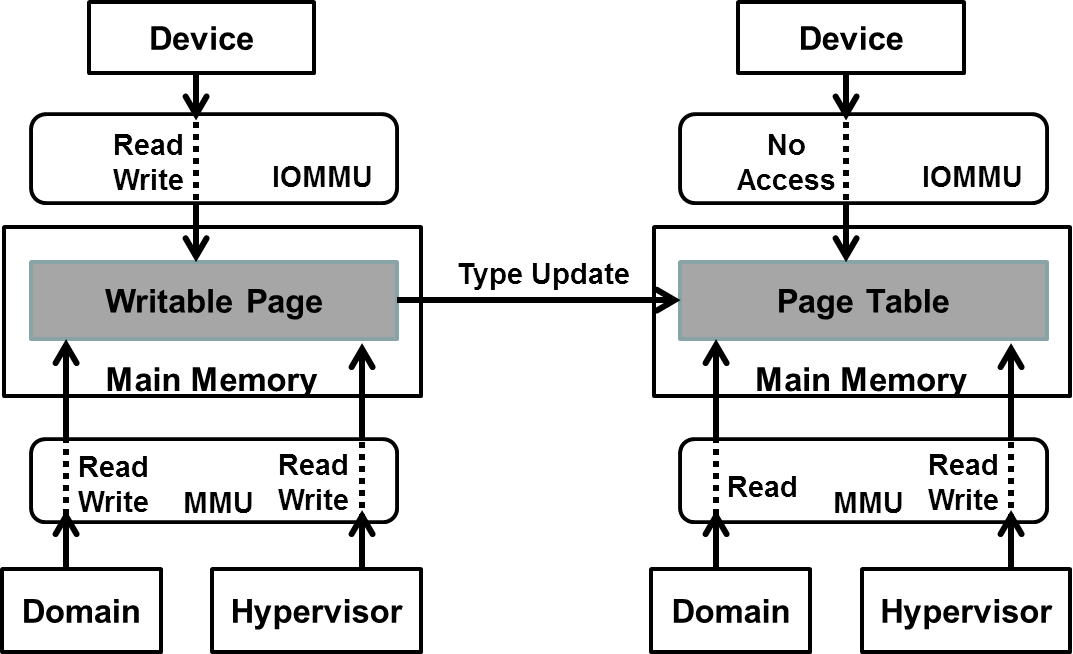
\includegraphics[width=0.5\textwidth]{image/translation/wr2pt.png} \\
\caption{a page type update from writable to page-table}
\label{fig:wr2pt}
\end{figure}

In a nutshell, page type updates as frequently occurs during processes creation/destruction, will force Xen to unmap/map the page from I/O page table and thus causing many IOTLB-flushes. As an IOTLB-miss requires a new page-walk for translation that can result in several consecutive accesses to memory, until the translation is done and the physical host address is resolved, a DMA transaction cannot be completed, which thereby may lead to a bad effect on I/O performance. It can be concluded that Xen has sacrificed I/O performance due to the safety reason. Because of that, we are motivated to reduce as many IOTLB misses as possible while retain the safety.
